\begin{tcolorbox}[posterbox]
\SectionTitle{Behavioral Results: Distance \& Direction}
\SmallText
Participants monitored and reported numerical changes.
\begin{itemize}
  \item \textbf{Distance effect:} RT decreased as numerical distance increased (Dist~3 faster than Dist~1), consistent with the standard distance effect.
  \item \textbf{Directional asymmetry:} Accuracy was significantly higher for Decreasing vs.\ Increasing changes.
  \item \textbf{Data included:} 24 participants, 5184 change trials for accuracy, and 4247 correct change trials with valid RT.
\end{itemize}

\begin{center}
  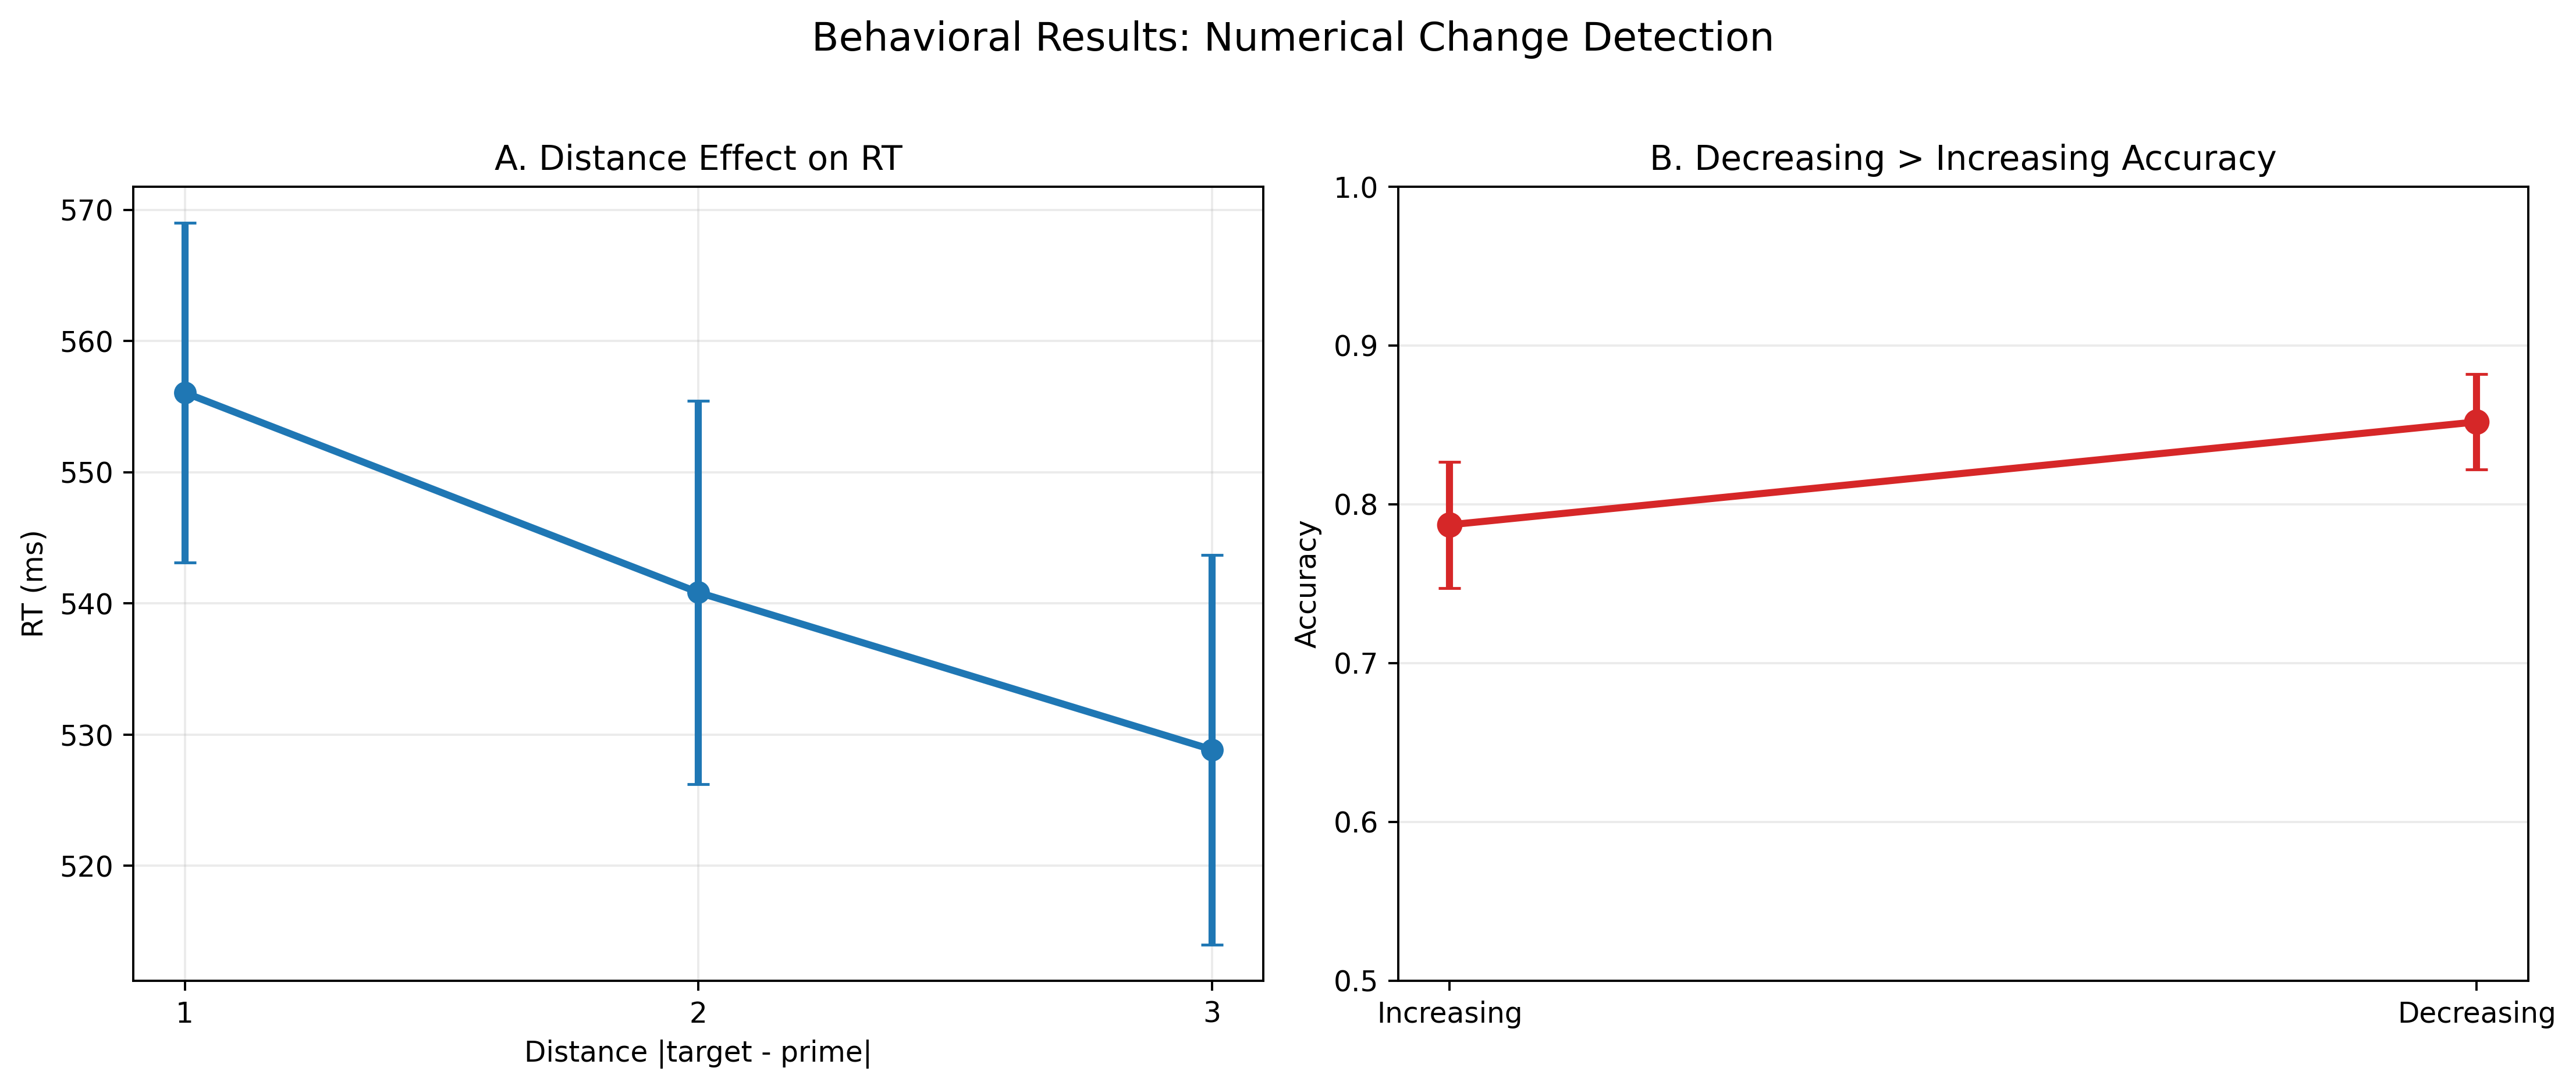
\includegraphics[width=0.90\linewidth, height=9in, keepaspectratio]{../docs/assets/poster_plots/behavioral/behavior_poster_main.png}
\end{center}

\begin{itemize}
  \item \textbf{RT distance effect:} log-RT GEE slope $b=-0.0261$, $SE=0.0033$, $p=5.31{\times}10^{-15}$ ($\sim$2.57\% faster per +1 distance).
  \item \textbf{Accuracy direction effect:} OR(Dec vs.\ Inc) $=1.596$, 95\% CI [1.339, 1.904], $p=1.96{\times}10^{-7}$.
  \item \textbf{Subject-level (two-sided):} RT slope $=-13.60$ ms/step ($p=3.05{\times}10^{-7}$); accuracy D$-$I $=0.0648$ ($p=7.67{\times}10^{-5}$).
\end{itemize}
\end{tcolorbox}

\vspace{0.06in}

\begin{tcolorbox}[posterbox]
\SectionTitle{Frontal Mismatch Negativity (MMN)}
\SmallText
\begin{itemize}
  \item Active monitoring recruited robust frontal MMN at Fz, peaking at $\sim$100--120 ms---indexing automatic numerical change detection.
  \item \textbf{Directional asymmetry:} Decreasing changes (red) elicited stronger, later MMN than Increasing (green), suggesting higher neural cost for quantity reduction.
  \item \textbf{Distance effect:} MMN amplitude scaled with numerical distance (Dist~3 $>$ Dist~1), mirroring behavioral accuracy.
\end{itemize}

\begin{center}
\begin{tabular}{cc}
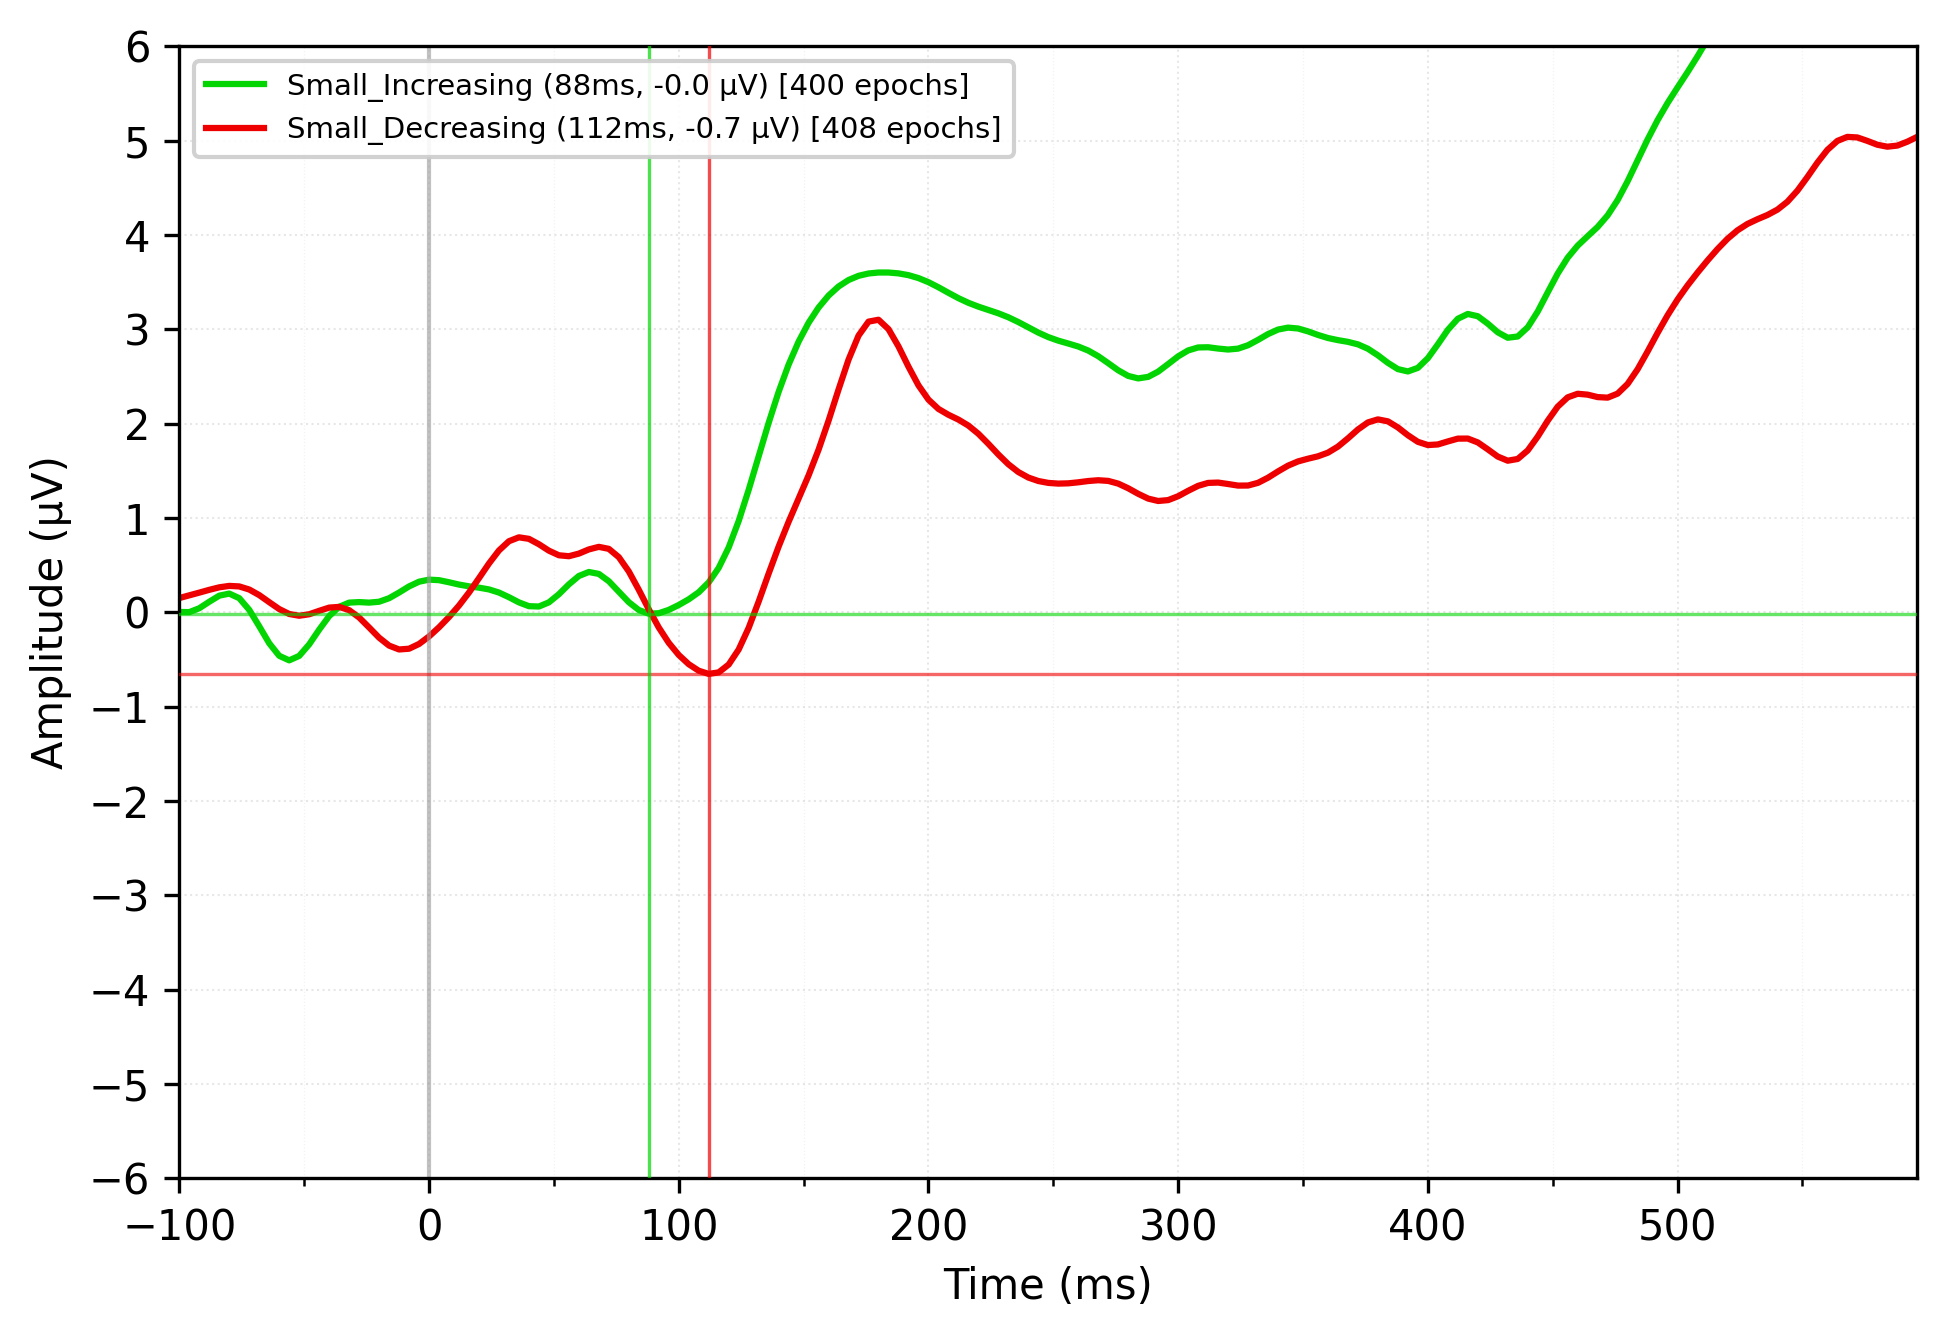
\includegraphics[width=0.45\linewidth, height=7in, keepaspectratio]{../docs/assets/plots/small_increasing_vs_decreasing_ACC1/small_increasing_vs_decreasing_ACC1-Fz-no_topo.png} &
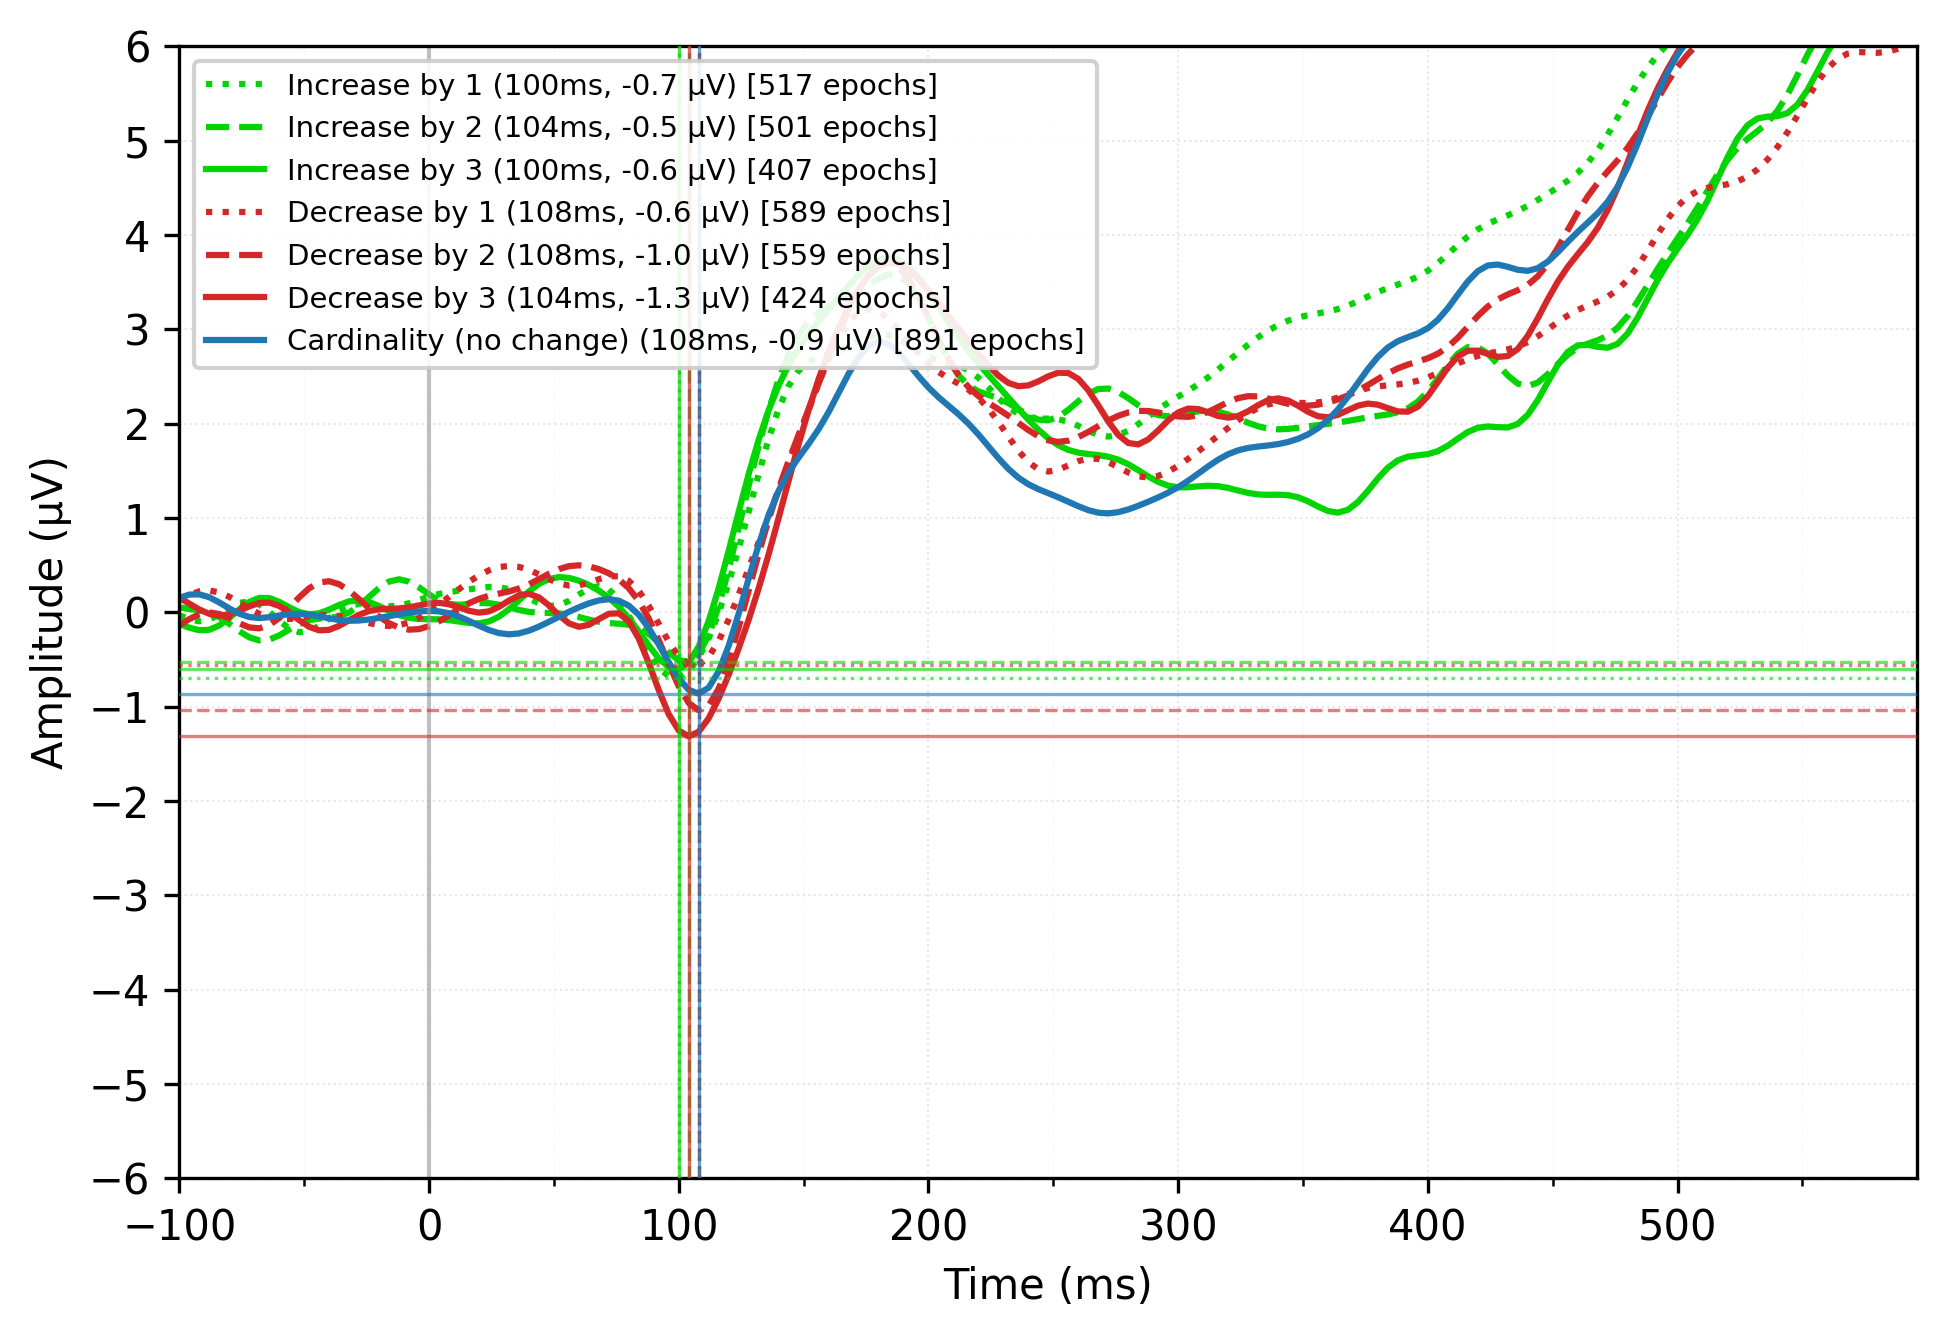
\includegraphics[width=0.45\linewidth, height=7in, keepaspectratio]{../docs/assets/plots/increase_decrease_123_ACC1/increase_decrease_123_ACC1-Fz-no_topo.png} \\
\end{tabular}
\end{center}
\SmallText
\textbf{Fig. 3.} Fz no-topo overlays for direction and distance effects.
\end{tcolorbox}

\vspace{0.06in}

\begin{tcolorbox}[posterbox]
\SectionTitle{Posterior N1: Direction Asymmetry}
\SmallText
\begin{itemize}
  \item Posterior N1 (bilateral POT) was \textbf{larger for Increasing} than Decreasing changes---opposite to frontal MMN---revealing a frontal/posterior dissociation in numerical change processing.
  \item P1--N1 peak-to-peak amplitude grew with numerical distance in both directions, paralleling MMN distance scaling.
\end{itemize}

\begin{center}
  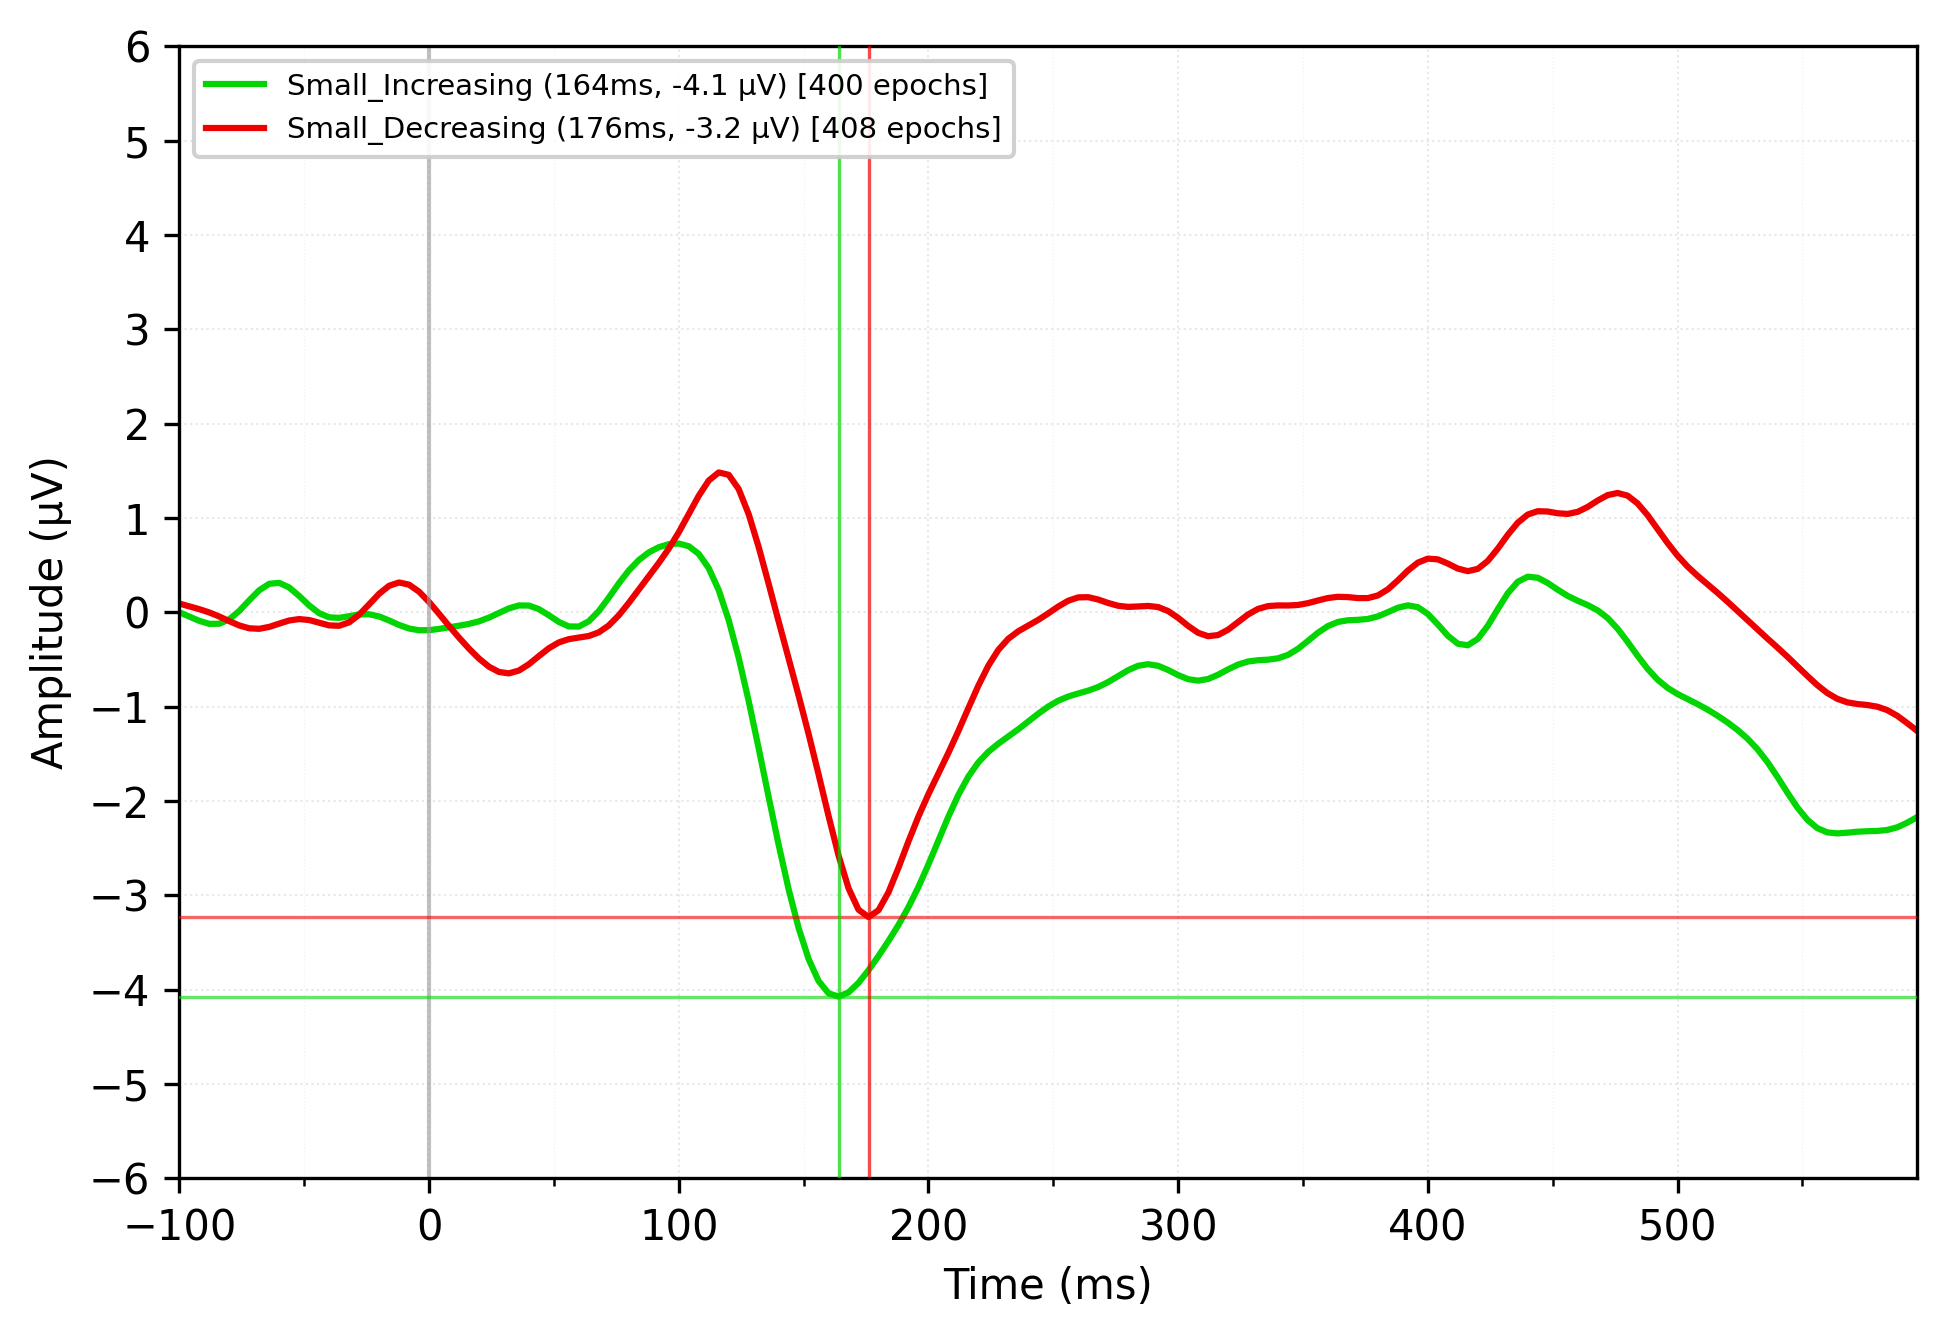
\includegraphics[width=0.86\linewidth, height=7in, keepaspectratio]{../docs/assets/plots/small_increasing_vs_decreasing_ACC1/small_increasing_vs_decreasing_ACC1-N1-no_topo.png}
\end{center}
\SmallText
\textbf{Fig. 4.} N1 no-topo: Increasing vs.\ Decreasing direction effect (bilateral POT).
\end{tcolorbox}
